\documentclass[11pt,a4paper]{article}
\usepackage[utf8]{inputenc}
\usepackage{natbib}
\usepackage{authblk}

%\VignetteIndexEntry{Learning how to use the niche metric functions (former 'resniche' package)}
%\VignettePackage{indicspecies}

\title{An example of usage of the niche metric functions (former 'resniche' package)}
\author[1]{Miquel De Cáceres}
\affil[1]{CTFC - Centre Tecnològic Forestal de Catalunya. Catalonia, Spain}
\author[2]{Oriol Lapiedra}
\author[2]{Daniel Sol}
\affil[2]{CREAF - Centre for Ecological Research and Applied Forestries, Catalonia, Spain}

\usepackage{Sweave}
\begin{document}
\Sconcordance{concordance:PigeonExample.tex:PigeonExample.Rnw:%
1 15 1 1 0 4 1 1 4 1 1 1 2 1 0 1 1 3 0 2 2 7 0 1 2 1 1 1 2 %
12 0 1 2 1 3 6 0 1 2 4 1 1 2 1 0 1 1 6 0 2 1 7 0 1 2 8 1 1 %
2 7 0 1 1 7 0 1 2 1 3 2 0 1 1 6 0 2 1 7 0 1 2 7 1 1 2 7 0 1 %
1 7 0 1 2 5 1 1 3 31 0 1 2 1 3 27 0 1 2 7 1 1 2 1 0 1 1 11 %
0 2 1 12 0 1 2 2 1 1 2 11 0 1 2 6 1 1 2 1 0 1 1 5 0 2 1 6 0 %
1 2 4 1 1 2 1 0 1 1 3 0 2 2 11 0 1 2 3 1 1 2 1 0 1 1 3 0 2 %
2 6 0 1 1 6 0 2 2 1 0 1 1 6 0 2 1 7 0 2 2 11 0 1 2 4 1}

\maketitle
\tableofcontents

\section{Introduction}
In this document we show how to use the functions described in \citep{DeCaceres2011} by following an example of dietary preferences in pigeons belonging to two populations (Moià and Barcelona) in Catalonia (north east of Spain). We begin by loading the library and the data:
\begin{Schunk}
\begin{Sinput}
> library(indicspecies)
> data(pigeons)
\end{Sinput}
\end{Schunk}
The data consists of three items: the resource use matrix for each pigeon population and the matrix of dissimilarities between pairs of resources (seeds). 
\begin{Schunk}
\begin{Sinput}
> ls()
\end{Sinput}
\begin{Soutput}
[1] "dfood"          "diet.barcelona" "diet.moia"     
\end{Soutput}
\end{Schunk}
\section{Resemblance between diet resources}
Before starting any resource niche calculation, we can inspect the matrix of dissimilarities between the $r=6$ resources, $\mathbf{D}$:
\begin{Schunk}
\begin{Sinput}
> dfood
\end{Sinput}
\begin{Soutput}
               Oats      Peas   Popcorn       Soy Sunflower
Peas      0.7029375                                        
Popcorn   0.3706196 0.5070959                              
Soy       0.7738801 0.6645980 0.8638219                    
Sunflower 0.7656489 0.9773428 0.8784905 0.8669801          
Wheat     0.3948828 0.5705974 0.2836482 0.7740283 1.0000000
\end{Soutput}
\end{Schunk}
These can be summarized using a dendrogram. For example:
\begin{Schunk}
\begin{Sinput}
> plot(hclust(dfood, method="average"), h=-1, xlab="", 
+      ylab="Distance", main="", sub="", ylim=c(0.2,1))
\end{Sinput}
\end{Schunk}
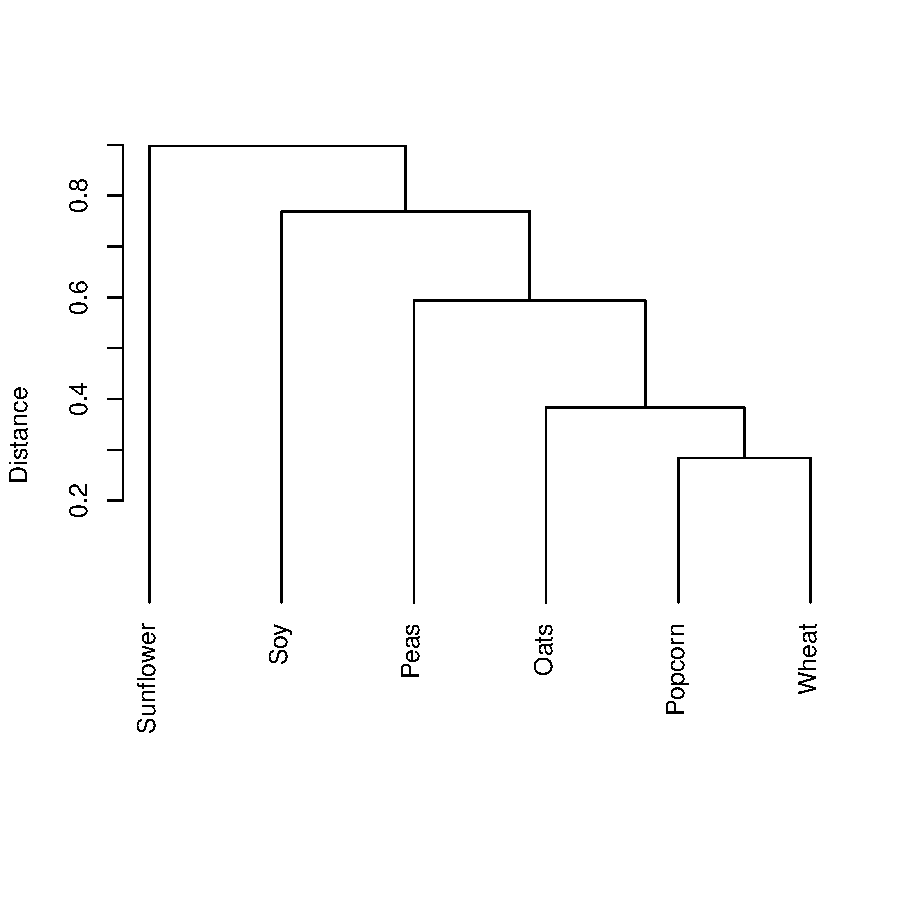
\includegraphics{PigeonExample-005}

Some seeds are quite similar (e.g. popcorn, wheat or oats), whereas sunflower differs substantially from all other resources.
\section{Resource niche analysis at the population level}
\subsection{Resource use of populations}
We begin by showing the resource use data for pigeons of Barcelona and Moia, expressed as proportions (i.e., the vector $\mathbf{f}$ for each population):
\begin{Schunk}
\begin{Sinput}
> diet.pop.barcelona = colSums(diet.barcelona)
> round(diet.pop.barcelona/sum(diet.pop.barcelona), dig=3)
\end{Sinput}
\begin{Soutput}
     Oats      Peas   Popcorn       Soy Sunflower     Wheat 
    0.049     0.001     0.028     0.024     0.455     0.442 
\end{Soutput}
\begin{Sinput}
> diet.pop.moia = colSums(diet.moia)
> round(diet.pop.moia/sum(diet.pop.moia), dig=3)
\end{Sinput}
\begin{Soutput}
     Oats      Peas   Popcorn       Soy Sunflower     Wheat 
    0.002     0.018     0.091     0.045     0.054     0.791 
\end{Soutput}
\end{Schunk}

Whereas pigeons in Moià feed almost exclusively on wheat, those of Barcelona combine wheat and sunflower seeds.

\subsection{Niche breadth in populations}
We will determine the resource niche breadth of each of the two populations as \citep{DeCaceres2011}: 
\[
B_{pop} = (1/2)\sum_{j=1}^r\sum_{k=1}^r{f_jf_kd_{jk}}
\]
We first conduct our calculations without taking into account the resemblance between resources (which is equal to stating that $d_{jk}=1$ in all cases):
\begin{Schunk}
\begin{Sinput}
> nichevar(P=diet.barcelona, mode="single")
\end{Sinput}
\begin{Soutput}
              B        LC        UC
Niche 0.2966578 0.2706666 0.3345246
\end{Soutput}
\begin{Sinput}
> nichevar(P=diet.moia, mode="single")
\end{Sinput}
\begin{Soutput}
              B        LC        UC
Niche 0.1807663 0.1048379 0.2634922
\end{Soutput}
\end{Schunk}
In general, we can say that the niche breadth of the population in Moià is smaller than the niche breadth of the population in Barcelona. If we repeat the same calculations with the matrix of resource resemblance, we realize that the niche breadth of both populations becomes smaller:
\begin{Schunk}
\begin{Sinput}
> popvar.barcelona = nichevar(P=diet.barcelona, D=dfood, 
+                             mode="single")
> popvar.barcelona
\end{Sinput}
\begin{Soutput}
              B       LC        UC
Niche 0.2453822 0.233744 0.2573655
\end{Soutput}
\begin{Sinput}
> popvar.moia= nichevar(P=diet.moia, D=dfood, mode="single")
> popvar.moia
\end{Sinput}
\begin{Soutput}
              B         LC        UC
Niche 0.0853328 0.02985418 0.1737896
\end{Soutput}
\end{Schunk}
The reason is that the first analysis was assuming that all resources were equally (and maximally) distinct, while the second analysis accounts for the similarity between some resources. Moreover, note that the niche breadth of Moià has decreased more than the niche breadth of Barcelona. This reflects that the resources being used by pigeons of Moià are more similar than the resources used by pigeons of Barcelona.

\subsection{Overlap between populations}
We can now calculate the niche overlap between the two pigeon populations:
\[
O_{12} = \frac{\sum_{j=1}^r\sum_{k=1}^r{f_{1j}f_{2k}(1-d_{jk}^2)}}{\sqrt{\sum_{j=1}^r\sum_{k=1}^r{f_{1j}f_{1k}(1-d_{jk}^2)}\sum_{j=1}^r\sum_{k=1}^r{f_{2j}f_{2k}(1-d_{jk}^2)}}}
\]
Using function \texttt{nicheoverlap}:
\begin{Schunk}
\begin{Sinput}
> nicheoverlap(P1=diet.barcelona, P2=diet.moia, mode="single")
\end{Sinput}
\begin{Soutput}
                O        LC        UC
Overlap 0.7419319 0.4624398 0.9222248
\end{Soutput}
\begin{Sinput}
> nicheoverlap(P1=diet.barcelona, P2=diet.moia, mode="single", D = dfood)
\end{Sinput}
\begin{Soutput}
                O        LC        UC
Overlap 0.7912472 0.5516827 0.9581053
\end{Soutput}
\end{Schunk}
If we include the resemblance between resources, the degree of overlap increases, for the same reason that we obtained smaller niche breadth statistics when resemblances were included.

\section{Resource niche analysis at the individual level}
In this section, we perform a resource niche analysis at individual level. In particular, we are interested in assessing how much the resource niche of individuals differs from that of their corresponding population. For this, we need to calculate a measure of the degree of individual specialization. 
\subsection{Resource use of individuals}
We begin by showing the resource use data for all \texttt{23} pigeons in the sample from the Barcelona population, expressed as proportions (i.e., matrix $\mathbf{F}$ for Barcelona):
\begin{Schunk}
\begin{Sinput}
> round(sweep(diet.barcelona, 1, FUN="/", 
+             rowSums(diet.barcelona)), dig=3)
\end{Sinput}
\begin{Soutput}
    Oats  Peas Popcorn   Soy Sunflower Wheat
1  0.000 0.000   0.000 0.000     0.020 0.980
2  0.000 0.000   0.000 0.000     1.000 0.000
3  0.000 0.000   0.000 0.000     1.000 0.000
4  0.025 0.000   0.153 0.000     0.000 0.822
5  0.000 0.000   0.000 0.000     0.965 0.035
6  0.000 0.023   0.136 0.000     0.648 0.193
7  0.000 0.000   0.000 0.000     0.795 0.205
8  0.042 0.000   0.000 0.000     0.000 0.958
9  1.000 0.000   0.000 0.000     0.000 0.000
10 0.014 0.000   0.000 0.000     0.014 0.973
11 0.000 0.000   0.000 0.000     0.350 0.650
12 0.000 0.000   0.000 0.000     0.047 0.953
13 0.000 0.000   0.000 0.000     0.437 0.562
14 0.000 0.000   0.000 0.000     0.389 0.611
15 0.000 0.000   0.000 0.549     0.451 0.000
16 0.000 0.000   0.000 0.000     0.913 0.087
17 0.000 0.000   0.113 0.075     0.755 0.057
18 0.000 0.000   0.043 0.000     0.743 0.214
19 0.000 0.000   0.000 0.000     0.667 0.333
20 0.000 0.000   0.000 0.000     0.367 0.633
21 0.000 0.000   0.000 0.000     0.910 0.090
22 0.000 0.000   0.019 0.019     0.786 0.175
23 0.442 0.000   0.000 0.000     0.000 0.558
\end{Soutput}
\end{Schunk}
We see that most individuals in Barcelona feed on either sunflower or wheat, but there are some individuals (like pigeon 9) which prefer oats. Now we display the resource use data for the \texttt{19} pigeons representing the population in Moià (i.e., matrix $\mathbf{F}$ for Moià):
\begin{Schunk}
\begin{Sinput}
> round(sweep(diet.moia, 1, FUN="/", 
+             rowSums(diet.moia)), dig=3)
\end{Sinput}
\begin{Soutput}
    Oats  Peas Popcorn   Soy Sunflower Wheat
1  0.000 0.000   0.000 0.324     0.000 0.676
2  0.000 0.000   0.000 0.012     0.000 0.988
3  0.000 0.000   0.000 0.000     0.000 1.000
4  0.000 0.000   0.000 0.000     0.000 1.000
5  0.000 0.000   0.000 0.000     0.000 1.000
6  0.000 0.000   0.267 0.000     0.000 0.733
7  0.000 0.000   0.319 0.000     0.000 0.681
8  0.027 0.311   0.041 0.000     0.000 0.622
9  0.000 0.000   0.000 0.000     0.000 1.000
10 0.000 0.000   0.148 0.000     0.000 0.852
11 0.000 0.000   0.200 0.000     0.000 0.800
12 0.000 0.000   0.235 0.000     0.000 0.765
13 0.000 0.000   0.000 0.000     0.000 1.000
14 0.000 0.000   0.119 0.339     0.136 0.407
15 0.000 0.000   0.000 0.000     0.000 1.000
16 0.000 0.000   0.000 0.000     0.000 1.000
17 0.000 0.000   0.430 0.000     0.000 0.570
18 0.000 0.000   0.000 0.000     0.583 0.417
19 0.000 0.000   0.000 0.000     1.000 0.000
\end{Soutput}
\end{Schunk}
Many pigeons from Moià feed on wheat seeds almost exclusively, but some of them have broader preferences. 

\subsection{Measuring the degree of individual specialisation}
We begin our resource niche analysis by calculating the niche breadth of each individual in the population, $B_i$:
\[
B_i = (1/2)\sum_{j=1}^r\sum_{k=1}^r{f_{ij}f_{ik}d_{jk}}
\]
We calculate the values for the individuals of both populations:
\begin{Schunk}
\begin{Sinput}
> indvar.barcelona<-nichevar(P=diet.barcelona, D=dfood)
> summary(indvar.barcelona)
\end{Sinput}
\begin{Soutput}
       B          
 Min.   :0.00000  
 1st Qu.:0.01755  
 Median :0.08153  
 Mean   :0.11168  
 3rd Qu.:0.19890  
 Max.   :0.24609  
\end{Soutput}
\begin{Sinput}
> indvar.moia<-nichevar(P=diet.moia, D=dfood)
> summary(indvar.moia)
\end{Sinput}
\begin{Soutput}
       B          
 Min.   :0.00000  
 1st Qu.:0.00000  
 Median :0.01015  
 Mean   :0.04031  
 3rd Qu.:0.01861  
 Max.   :0.24306  
\end{Soutput}
\end{Schunk}
Most individuals have niche breadths that are smaller than the niche breadth of their corresponding population, although a few individuals in Moià have niche breadths larger than the population value. A niche breadth equal to zero indicates that only one resource is exploited. 

We can compare the niche breadth values of the two populations using a non-parametric test.
\begin{Schunk}
\begin{Sinput}
> wilcox.test(indvar.barcelona$B, indvar.moia$B)
\end{Sinput}
\begin{Soutput}
	Wilcoxon rank sum test with continuity correction

data:  indvar.barcelona$B and indvar.moia$B
W = 328, p-value = 0.005446
alternative hypothesis: true location shift is not equal to 0
\end{Soutput}
\end{Schunk}
The Wilcoxon test confirms that the niche breadth of pigeons in Barcelona is generally higher than that of pigeons in Moià, as we saw at the population level.

In order to calculate the degree of individual specialization, \citet{Bolnick2002} defined WIC/TNW, i.e. the ratio between the within individual component (i.e. average niche width) and the total niche width of the population. Similarly we define the following specialization measure, that takes into account the resemblance between resources:
\[
S_{pop} = \frac{\sum_{i=n}^n{B_i}/n}{B_{pop}}
\]
where $B_i$ is the niche breadth of each individual, and $B_{pop}$ is the niche breadth of the population. Note that it is possible that $B_i$ values can be larger than $B_{pop}$. However, we do not expect the average of $B_i$ values to be larger than $B_{pop}$. If we calculate $S_{pop}$ for the two populations we have:
\begin{Schunk}
\begin{Sinput}
> Spec.barcelona = mean(indvar.barcelona$B)/popvar.barcelona$B
> Spec.barcelona
\end{Sinput}
\begin{Soutput}
[1] 0.4551234
\end{Soutput}
\begin{Sinput}
> Spec.moia = mean(indvar.moia$B)/popvar.moia$B
> Spec.moia
\end{Sinput}
\begin{Soutput}
[1] 0.4723618
\end{Soutput}
\end{Schunk}
Surprisingly, the degree of specialization in Moià seems slightly higher than that in Barcelona. To see whether this holds statistically, we can calculate the degree of specialization of each individual:
\[
S_i = \frac{B_i}{B_{pop}}
\]
which, in R, is:
\begin{Schunk}
\begin{Sinput}
> Spec.ind.barcelona = indvar.barcelona$B/popvar.barcelona$B
> Spec.ind.moia = indvar.moia$B/popvar.moia$B
\end{Sinput}
\end{Schunk}
Finally, we compare this two vectors in a Wilcoxon test:
\begin{Schunk}
\begin{Sinput}
> wilcox.test(Spec.ind.barcelona, Spec.ind.moia)
\end{Sinput}
\begin{Soutput}
	Wilcoxon rank sum test with continuity correction

data:  Spec.ind.barcelona and Spec.ind.moia
W = 277, p-value = 0.1392
alternative hypothesis: true location shift is not equal to 0
\end{Soutput}
\end{Schunk}
Which tells us that those differences in individual specialization are not statistically significant.

\subsection{Measuring the degree of overlap between individuals}
The idea of this section is to determine how much the niche of each individual overlaps with the niche of other individuals in the population. This can be done by calling function \texttt{nicheoverlap} in the `pairwise' mode:
\begin{Schunk}
\begin{Sinput}
> O.barcelona = nicheoverlap(diet.barcelona,D=dfood, mode="pairwise")
> O.moia = nicheoverlap(diet.moia,D=dfood, mode="pairwise")
\end{Sinput}
\end{Schunk}
These calls to \texttt{nicheoverlap} return a symmetric square matrix with as many rows and columns as individuals in the resource use data frame. Each cell value in the symmetric matrix is the overlap between two individuals of the population. Using these matrices we can derive the average overlap in each population:
\begin{Schunk}
\begin{Sinput}
> mean(O.barcelona[lower.tri(O.barcelona)])
\end{Sinput}
\begin{Soutput}
[1] 0.6726374
\end{Soutput}
\begin{Sinput}
> mean(O.moia[lower.tri(O.moia)])
\end{Sinput}
\begin{Soutput}
[1] 0.8438816
\end{Soutput}
\end{Schunk}
We can also calculate the average overlap between each individual and the remaining individuals in its population:
\begin{Schunk}
\begin{Sinput}
> O.barcelona.ind = (rowSums(O.barcelona)-1)/(nrow(O.barcelona)-1)
> summary(O.barcelona.ind)
\end{Sinput}
\begin{Soutput}
   Min. 1st Qu.  Median    Mean 3rd Qu.    Max. 
 0.5400  0.6028  0.6558  0.6726  0.7595  0.8055 
\end{Soutput}
\begin{Sinput}
> O.moia.ind = (rowSums(O.moia)-1)/(nrow(O.moia)-1)
> summary(O.moia.ind)
\end{Sinput}
\begin{Soutput}
   Min. 1st Qu.  Median    Mean 3rd Qu.    Max. 
0.09157 0.89920 0.90650 0.84390 0.90970 0.91130 
\end{Soutput}
\end{Schunk}
We substracted one in the numerator and denominator in order to exclude the target individual from the average (the overlap between a resource niche and itself is always one). Apparently, the individuals in Moià have a larger degree of overlap with individuals of their population than individuals in Barcelona. A non-parametric test seems to confirm this difference:
\begin{Schunk}
\begin{Sinput}
> wilcox.test(O.barcelona.ind, O.moia.ind)
\end{Sinput}
\begin{Soutput}
	Wilcoxon rank sum test with continuity correction

data:  O.barcelona.ind and O.moia.ind
W = 37, p-value = 4.549e-06
alternative hypothesis: true location shift is not equal to 0
\end{Soutput}
\end{Schunk}

\bibliographystyle{plainnat}
\bibliography{resniche}

\end{document}
